\documentclass[11pt,a4paper]{article}
\XeTeXlinebreaklocale "zh"
\XeTeXlinebreakskip = 0pt plus 1pt minus 0.1pt
\usepackage[top=1in,bottom=1in,left=1.25in,right=1.25in]{geometry}
\usepackage{float}
\usepackage{fontspec}
\newfontfamily\zhfont[BoldFont=STHeiti]{STFangsong}
\newfontfamily\zhpunctfont{STFangsong}
\setmainfont{Times New Roman}
\usepackage{indentfirst}
\usepackage{zhspacing}
\zhspacing

\usepackage[colorlinks=true]{hyperref}

% 代码展示
\usepackage{color}
\definecolor{bg}{rgb}{0.152941, 0.156863, 0.133333}
\usepackage{minted}
\usemintedstyle{monokai}
\setmonofont{DejaVuSansMono}

\usepackage{fancyvrb}  % 调整 Verbatim 中字体

% 调整 quotation 字体
\let\quotationOLD\quotation
\def\quotation{\quotationOLD\footnotesize}

\usepackage{pdfpages}  % 附上 pdf 版综合结果

\renewcommand{\figurename}{图 }  % 图片标题

\begin{document}

\title{实验三\ \ 频率计设计}
\author{无36$\quad$李思涵$\quad$2013011187}
\maketitle

\section{实验目的}
\begin{itemize}
  \item 掌握频率计的原理和设计方法。
\end{itemize}

\section{设计方案}
\subsection{原理说明}
本次实验中,主要任务在于实现频率计,并且该频率计要实现两个量程。下面是实验指导书中的原理说明。

\begin{quotation}
“频率计用于对一个未知频率的周期信号进行频率测量,在1s内对信号周期进行计数,即为此周期信号的频率。

频率计内部实现框图如下所示,其内部包括频率量程处理模块(10分频)、时钟频率产生模块、控制信号产生模块、十进制计数器模块、锁存器模块、译码显示模块等。

利用系统时钟产生1Hz的控制信号,在1s的时长内利用计数器对待测信号进行计数,将计数结果锁存(或者保存,不是指latch)并输出到数码管中显示。

其中频率量程模块负责根据设定的量程控制信号决定是否对输入信号进行10分频;
系统时钟模块根据外部输入的参考时钟产生标准 1Hz 的控制信号;
控制信号产生模块产生计数所需的使能、清零信号以及保存测量结果所需的锁存信号和扫描显示所需的扫描时钟信号;
十进制计数模块在计数使能、清零信号控制下对外部输入信号(或其10分频信号)在1s周期内对其进行计数操作;
锁存器模块在计数完成之后对计数结果进行锁存,保存上一测量周期的测量结果;
译码显示模块将测量结果输出到LED数码管显示,采用扫描的方式实现多位数据的同时显示。”
\end{quotation}

从上面可以看出,频率计主要由以下几个部分组成:

\begin{description}
  \item[分频器] 有两个档位,高频档输出 10 分频后的信号,低频档则直接输出原信号。
  \item[系统时钟模块] 利用 V10 端口提供的 100MHz 时钟生成 1Hz 的控制信号和 1kHz 的数码管扫描信号。
  \item[控制信号产生模块] 利用 1Hz 时钟对计数器,锁存器产生控制信号。
  \item[4位十进制计数器] 对信号进行计数。
  \item[锁存器模块] 在 Lock 信号有效时锁定输出,否则透明输出计数器的值。这么做是为了在数码管上实现 “动态计数” 与 “显示频率” 两个状态相互转换的效果。
  \item[译码显示模块] 用数码管显示当前的计数器值/当前信号频率,并用 LED 灯指示当前频率。
\end{description}

故只要分别实现这几个模块,并将它们正确地连接起来,便可以实现频率器。

不过要注意这里所说的模块并不一定要实现成一个独立的 module,只需要实现其功能便可以了。

\subsection{框图}
图~\ref{fig:频率计} 表示了频率计的结构。可以看到,各个模块都是以控制信号模块为中心的。

图~\ref{fig:频率计测试系统} 则代表了频率计测试系统的结构。其中 Testmode[1:0] 用于控制测试信号的频率,其为四个不同值时会产生四个不同频率的信号,从而达到测试的目的。

\begin{figure}[htb]
  \centering
    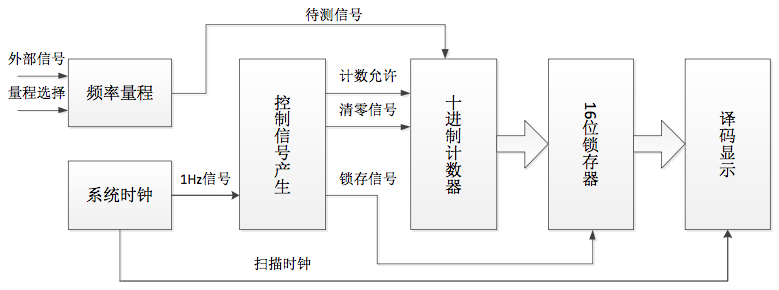
\includegraphics[width=\textwidth]{exp3_freq_meter}
  \caption{频率计}
  \label{fig:频率计}
\end{figure}

\begin{figure}[htb]
  \centering
    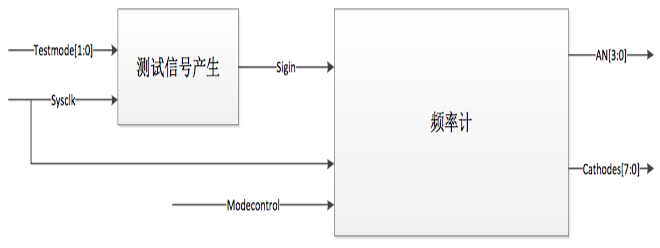
\includegraphics[width=\textwidth]{exp3_freq_meter_tb}
  \caption{频率计测试系统}
  \label{fig:频率计测试系统}
\end{figure}

\section{关键代码}

\subsection{分频器的实现}

\begin{minted}[bgcolor=bg, linenos=true, fontsize=\footnotesize]{verilog}
module divider(new_signal, range, signal);

output new_signal;
input range, signal;

parameter RATIO = 10,
          HALF_RATIO = RATIO / 2;

reg [3:0] counter;

reg divided_signal = 0;
assign new_signal = (range ? divided_signal : signal);

always @(posedge signal) begin
    // Use a higher range.
    if (counter >= HALF_RATIO) begin
        counter <= 1;
        divided_signal <= ~divided_signal;  // Flip.
    end else begin
        counter <= counter + 1'b1;
    end
end

endmodule
\end{minted}

可以看到,10-分频器可以用计数器实现,即每 5 个时钟周期反转输出时钟。而量程选择则可以用多路选择器,即 verilog 代码中的三目表达式轻松地实现。

\subsection{频率计中控制部分的实现}

\begin{minted}[bgcolor=bg, linenos=true, fontsize=\footnotesize]{verilog}
// Central control.
wire [15:0] num;
wire reset_n;
counter #(16, 9999) four_bit_counter(num, new_signal, 1'b1, reset_n);


reg [1:0] state = 0, next_state = 0;
always @(state, control_clk) begin
    case (state)
        2'd0: next_state = (control_clk ? 2'd1 : 2'd0);
        2'd1: next_state = 2;
        2'd2: next_state = (control_clk ? 2'd2 : 2'd0);
        default: next_state = 0;
    endcase
end

assign reset_n = (state == 1 ? 1'b0 : 1'b1);

always @(posedge clk) begin
    state <= next_state;
end

reg lock = 0;
always @(posedge control_clk) begin
    if (lock) begin
        lock <= 1'b0;
    end else begin
        lock <= 1'b1;
        saved_num = num;
    end
end

reg [15:0] saved_num;
wire [15:0] led_num = (lock ? saved_num : num);  // Number to be displayed on the LED.
\end{minted}

频率计中的控制部分主要包括了对 reset\_n 信号的控制(十分捉急地用状态机实现 orz),lock 信号的控制,以及根据 lock 的值选择输出到数码管的数字。


\section{文件清单}

\begin{Verbatim}[fontsize=\scriptsize]
exp2
└── freq_meter
    ├── divider.v
    ├── freq_meter.v
    ├── freq_meter_tb.v
    ├── Makefile
    ├── siginput.v
    ├── sim
    ├── top.bit
    ├── top.ucf
    └── top.v

common
├── bcd7.v
├── counter.v
├── led.v
└── watchmaker.v
\end{Verbatim}

其中 Makefile 用来构建仿真程序,sim 文件为 Icarus Verilog 生成的仿真程序。


\section{仿真结果及分析}
使用的仿真工具为:Icarus Verilog 0.9.7。

仿真结果如下:

\VerbatimInput[fontsize=\scriptsize, numbers=left]
{../../exp3/freq_meter/result.txt}

因为模拟周期过长,所以只展示了仿真结果的前 51 行。从其中可以看到,1kHz 的扫描信号确实起到了作用(从 anodes 的变化中可以看出),而数码管在这个状态下也确实实现了透明显示计数器值的功能(从 cathodes 的变化可以看出)。

\section{综合情况}
见附页。

\section{硬件调试情况}

刚开始的时候,由于把计数器放到一个模块中实现了,所以在清零时遇到了一些麻烦:如何产生一个计数器清零脉冲信号?后来还是用状态机实现了,但是显得比较臃肿。最后得到的经验是:对于计数器这样的简单元件,没有太大的必要放入一个模块,直接在 RTL 级实现会比较方便。

后来虽然实现了一个可以正常工作的版本,但是当时却没有注意到实验指导书中提到的 “Lock 信号有效时输出锁定,否则,输出透明显示计数器值”。后来经舍友提醒才发现 orz

最后在狼狈地代码中加入了 lock 变量,才达到了要求……以后在开始实现以前一定要看清楚要求,这样才不会被坑 orz。

Cheers \textasciitilde

\includepdf[pages={-}]{freq_meter.pdf}

\end{document}

